\chapter{Reliability}
\section{Esercizio 1}
Calcolare \textbf{Reliability} e \textbf{MTTF} per il sistema il cui Reilability Block Diagram è rappresentato nell'immagine sottostante. Assumere che tutti i componenti sono identici e falliscono randomicamente con tasso di fallimento \textit{$\lambda$}.
\begin{figure}[H]
	\centering
	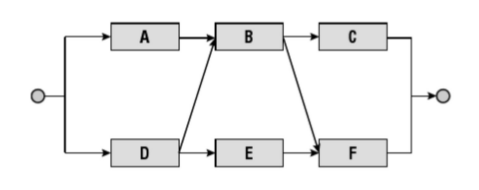
\includegraphics[width=1\textwidth]{img/hw5/es1.png}
	\caption{\textit{Reliability Block Diagram Es.1}}
\end{figure}
\subsection{Svolgimento}
Dalla traccia si evince che la \textit{reliability} di un singolo blocco del sistema in questione ha andamento esponenziale ed è:
\begin{equation*}
	R_i = e^{-\lambda*t}
\end{equation*}
\subsubsection{Success Diagram}
Non è ancora possibile riconoscere una serie da un parallelo in questo caso, quindi una prima cosa da fare è ricavare un \textit{success diagram}, ovvero un sistema composto da un parallelo di serie. Le serie sono anche dette \textit{success path} e coincidono con tutti i percorsi possibili dall'ingresso all'uscita del sistema. 
\begin{figure}[H]
	\centering
	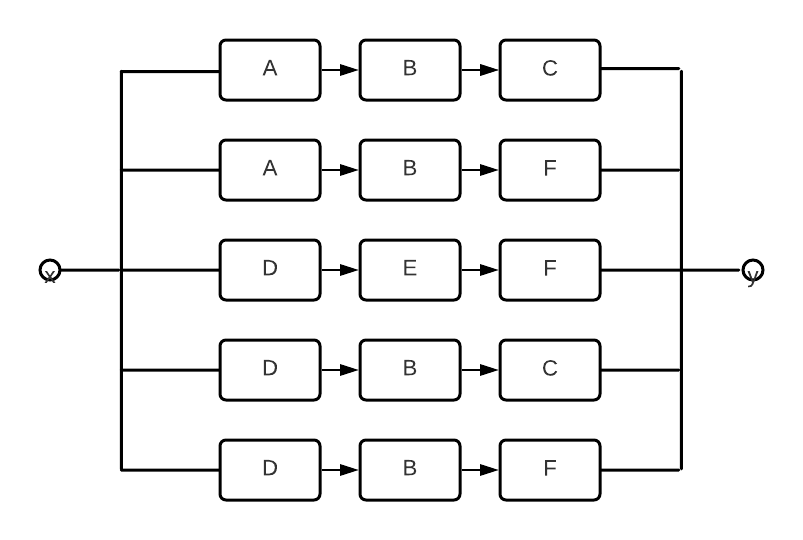
\includegraphics[width=0.7\textwidth]{img/hw5/success_diag.png}
	\caption{\textit{Success Diagram Es.1}}
\end{figure}
\begin{equation*}
	Rsys \leq 1 - \prod_{i=1}^{N}(1 - Rpath_i)
\end{equation*}
Con $N$ pari al numero di serie del diagramma, e $Rpath_i$ la reliability del path i-esimo.
\\Nel caso specifico dell'esercizio:
\begin{equation*}
	Rsys \leq 1 - [(1 - R_A*R_B*R_C)*(1-R_A*R_B*R_F)*(1-R_D*R_E*R_F)*(1-R_D*R_B*R_C)*(1-R_D*R_B*R_F)]
\end{equation*}
In questo modo è possibile ricavare agevolmente una reliability che sarà un upper bound per quella effettiva del sistema. Difatti i vari path non sono tra di loro indipendenti, dato che il fallimento di un blocco potrebbe interessare più di una serie.
\begin{equation*}
	Rsys \leq 1 - (1 - e^{-3\lambda*t})^{5}
\end{equation*}
\subsubsection{Conditioning}
La tecnica del \textbf{conditioning} consente di ricavare la reliability di un sistema facendo uso della formula del teorema di Bayes:
\begin{equation*}
	P(A) = \sum_{i = 1}^{N}P(A/B_i)P(B_i)
\end{equation*}
In poche parole, dato il sistema, viene supposto che uno dei suoi componenti $R_m$ (quello più critico per l'analisi) sia fallito o meno. Otteniamo quindi due versioni del diagramma iniziale:
\begin{enumerate}
	\item \textit{con componente selezionato up (circuito chiuso)}.
	\item \textit{con componente selezionato down (circuito aperto)}.
\end{enumerate}
\begin{equation*}
	Rsys = Rsys_1 + Rsys_2 = R_m*P(sys\,works|m\,up) + (1 - R_m)*P(sys\,works|m\,down)
\end{equation*}
\subsubsection{Conditioning sul blocco E}
\begin{figure}[H]
	\centering
	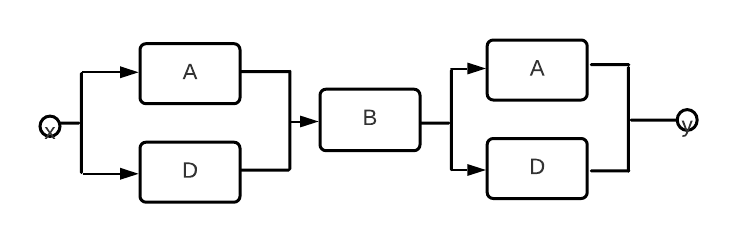
\includegraphics[width=0.7\textwidth]{img/hw5/e_down.png}
	\caption{\textit{Diagramma con Blocco E down Es.1}}
\end{figure}
Il sistema è composto da 2 paralleli in serie con il blocco B. La reliability totale può essere calcolata agevolmente sfruttando le formule di blocchi in serie e in parallelo.
\begin{equation*}
	Rsys_2 = (1-R_E)*P(sys\,works|E\,down)=
\end{equation*}
\begin{equation*}
	 = (1-R_E)*[[1-(1-R_A)*(1-R_E)]*R_B*[1-(1-R_C)*(1-R_F)]] =
\end{equation*}
\begin{equation*}
	= (1-e^{-\lambda*t})*[1-(1-e^{-\lambda*t})^{2}]^{2}*e^{-\lambda*t}=
\end{equation*}
\begin{equation*}
	= (1-e^{-\lambda*t})*[1-(1+e^{-2\lambda*t}-2e^{-\lambda*t})]^{2}*e^{-\lambda*t}=
\end{equation*}
\begin{equation*}
	= (1-e^{-\lambda*t})*[-e^{-2\lambda*t}+2e^{-\lambda*t}]^{2}*e^{-\lambda*t}=
\end{equation*}
\begin{equation*}
	= (1-e^{-\lambda*t})*[e^{-4\lambda*t}+4e^{-2\lambda*t}-4e^{-3\lambda*t}]*e^{-\lambda*t}=
\end{equation*}
\begin{equation*}
	= (1-e^{-\lambda*t})*[e^{-5\lambda*t}+4e^{-3\lambda*t}-4e^{-4\lambda*t}]=
\end{equation*}
\begin{equation*}
	= [e^{-5\lambda*t}+4e^{-3\lambda*t}-4e^{-4\lambda*t}] - [e^{-6\lambda*t}+4e^{-4\lambda*t}-4e^{-5\lambda*t}]=
\end{equation*}
\begin{equation*}
	= 4e^{-3\lambda*t}+5e^{-5\lambda*t}-e^{-6\lambda*t}
\end{equation*}
\begin{figure}[H]
	\centering
	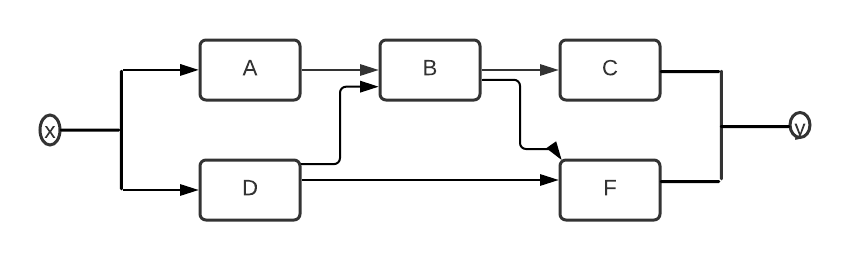
\includegraphics[width=0.7\textwidth]{img/hw5/e_up.png}
	\caption{\textit{Diagramma con Blocco E up Es.1}}
\end{figure}
\begin{equation*}
	Rsys_1 = R_E*P(sys\,works|E\,up)
\end{equation*}
Tuttavia il sistema così ottenuto deve ancora essere condizionato, visto che non essendo combinazione di serie e/o paralleli non è possibile ricavare immediatamente la probabilità condizionata.
\subsubsection{Conditioning sul blocco B - E up}
\begin{figure}[H]
	\centering
	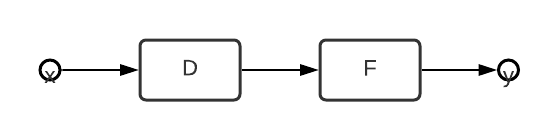
\includegraphics[width=0.7\textwidth]{img/hw5/b_down.png}
	\caption{\textit{Blocco E up e Blocco B down Es.1}}
\end{figure}
\begin{figure}[H]
	\centering
	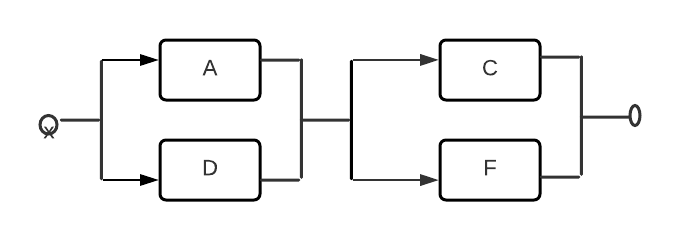
\includegraphics[width=0.7\textwidth]{img/hw5/b_up.png}
	\caption{\textit{Blocco E up e Blocco B up Es.1}}
\end{figure}
\begin{equation*}
	P(sys\,works|E\,up) = P(sys\,works|B\,down)*P(B\,down)+P(sys\,works|B\,up)*P(B\,up) =
\end{equation*}
\begin{equation*}
	= (1-R_B)*R_D*R_F + R_B*[1-(1-R_A)*(1-R_D)]*[1-(1-R_C)*(1-R_F)] =
\end{equation*}
\begin{equation*}
	= (1-e^{-\lambda*t})*e^{-2\lambda*t} + e^{-\lambda*t}*[1-(1-e^{-\lambda*t})^{2}]^{2} =
\end{equation*}
\begin{equation*}
	= e^{-2\lambda*t} - e^{-3\lambda*t} + e^{-\lambda*t}*[e^{-4\lambda*t}+4e^{-2\lambda*t}-4e^{-3\lambda*t}] =
\end{equation*}
\begin{equation*}
	= e^{-2\lambda*t} - e^{-3\lambda*t} + e^{-5\lambda*t}+4e^{-3\lambda*t}-4e^{-4\lambda*t} =
\end{equation*}
\begin{equation*}
	= e^{-2\lambda*t} + 3e^{-3\lambda*t} -4e^{-4\lambda*t} +e^{-5\lambda*t} 
\end{equation*}
Dunque otteniamo che :
\begin{equation*}
	Rsys_1 = e^{-\lambda*t}*[e^{-2\lambda*t} + 3e^{-3\lambda*t} -4e^{-4\lambda*t} +e^{-5\lambda*t}] =
\end{equation*}
\begin{equation*}
	 = e^{-3\lambda*t} + 3e^{-4\lambda*t} -4e^{-5\lambda*t} +e^{-6\lambda*t}
\end{equation*}
Quindi la \textbf{reliability totale} del sistema sarà:
\begin{equation*}
	Rsys = 4e^{-3\lambda*t}+5e^{-5\lambda*t}-e^{-6\lambda*t} + e^{-3\lambda*t} + 3e^{-4\lambda*t} -4e^{-5\lambda*t} +e^{-6\lambda*t} = 
\end{equation*}
\begin{equation*}
	 = 5e^{-3\lambda*t}+3e^{-4\lambda*t}+ e^{-5\lambda*t}
\end{equation*}
Mentre il \textbf{MTTF - Mean Time To Failure} è:
\begin{equation*}
	MTTF = \int_{0}^{\infty} Rsys(t)dt = \frac{5}{3\lambda}+\frac{3}{4\lambda}+\frac{1}{5\lambda}
\end{equation*}
\section{Esercizio 2}
\subsubsection{Svolgimento}
\section{Esercizio 3}
\subsubsection{Svolgimento}
\section{Esercizio 4}
\subsubsection{Svolgimento}
\section{Esercizio 5}
\subsubsection{Svolgimento}